% LKOS Working Notes - Revision 0.10.0
% arXiv-style technical report, single-column article.
% Cover is generated separately via HTML/Playwright (Template 03) and merged as page 0.
\documentclass[11pt,a4paper]{article}

\usepackage{geometry}
\geometry{a4paper, top=2.5cm, bottom=2.5cm, left=2.5cm, right=2.5cm}
% left == right (symmetry iron rule)

\usepackage{amsmath}
\usepackage{graphicx}
\usepackage{xcolor}
\usepackage{booktabs}
\usepackage{tabularx}
\usepackage{adjustbox}
\usepackage{enumitem}
\usepackage{microtype}
\usepackage{needspace}
\usepackage[normalem]{ulem}
\usepackage[htt]{hyphenat}   % allow hyphenation/breaking inside \texttt (long identifiers)
\usepackage{tikz}
\usetikzlibrary{arrows.meta,positioning}

% hyperref - ALWAYS last among content packages
\usepackage[
    colorlinks=true,
    linkcolor=blue,
    citecolor=darkgray,
    urlcolor=blue,
    bookmarks=true,
    bookmarksnumbered=true,
    unicode=true
]{hyperref}

\widowpenalty=10000
\clubpenalty=10000
\emergencystretch=3em        % resolve residual overfull boxes gracefully

\hypersetup{
    pdftitle={LKOS: A Local-First Knowledge Intelligence Engine with Corpus-Trained Semantic Retrieval, Typed Evidence, and Provenance-Preserving Incremental Indexing},
    pdfauthor={Bilal140202 (LKOS Project)},
    pdfsubject={Local-first knowledge intelligence: corpus-trained semantic retrieval, typed evidence, provenance-preserving incremental indexing},
    pdfkeywords={local-first, information retrieval, LSA, HNSW, approximate nearest neighbor, knowledge graph, provenance, SQLite, hybrid search}
}

\begin{document}

% ═══════════════════════════════════════════════════════
% NO TITLE PAGE IN .tex - Cover is generated separately
% via HTML/Playwright and merged as page 0.
% TOC must be the FIRST page of the body PDF.
% ═══════════════════════════════════════════════════════

\tableofcontents
\newpage

% ─────────────────────────────────────────────────────────
% Front matter (compact title block, not \maketitle), Abstract, §1, §2
% ─────────────────────────────────────────────────────────

\begin{center}
  {\LARGE\bfseries LKOS: A Local-First Knowledge Intelligence Engine with
  Corpus-Trained Semantic Retrieval, Typed Evidence, and
  Provenance-Preserving Incremental Indexing\par}
  \vspace{1.0em}
  {\normalsize LKOS Working Notes --- Revision 0.10.0\par}
  \vspace{0.4em}
  {\small Repository: \url{https://github.com/Bilal140202/lkos-system}
  \,\textperiodcentered\, License: MIT\par}
\end{center}

\vspace{0.6em}

\begin{abstract}
\noindent
LKOS (Local Knowledge Object System) is an offline, privacy-first knowledge
intelligence engine that transforms raw documents into structured, searchable,
relationally connected, versioned knowledge --- entirely on-device, with no
network access and no required language model. This paper describes the v0.10
architecture and its empirical evaluation. The system couples a canonical
SQLite substrate with structure-aware chunking, a \textbf{corpus-trained
latent-semantic embedding provider} (PPMI weighting + randomized truncated
SVD, deterministic by construction), hybrid retrieval via Reciprocal Rank
Fusion with a deterministic lexical-overlap reranker, multi-stage entity
resolution, an evidence layer with typed conflict taxonomy, typed
knowledge-graph construction with graph-correct deletion, and a durable job
system with exponential backoff and atomic claiming. Every derived artifact
carries provenance to its source span.

We report measurements on commodity hardware: semantic model training at
\textbf{0.06\,s per 2,400 chunks}, re-embedding at \textbf{22.9k chunks/s},
hybrid query latency \textbf{p50 7.4\,ms / p99 8.1\,ms} on a 200-document
library, and --- on a 16-query golden set with graded relevance judgments ---
\textbf{MRR 1.000 and nDCG@10 0.966} for the hybrid stack. v0.10 adds a
\textbf{deterministic in-process HNSW index} (Malkov \& Yashunin) for the
dense channel: on a 100,000-chunk clustered corpus (128-d) it reduces dense
p50 from 20.24\,ms (exact scan) to \textbf{0.42\,ms at measured recall@10
0.967} (ef=128; 0.30\,ms at 0.853 with ef=64), with an exact fingerprint-based
cache invalidation and a degrade-not-refuse policy past the former scan cap
(ADR-010). We additionally document twelve defects found and fixed through
adversarial self-audit and the project's own three-OS CI gate, including a
regex-greediness entity-extraction defect that merged distinct organizations,
a quadratic conflict-materialization pathology that we bound by capping
pairwise enumeration, and --- new in v0.10 --- two HNSW construction defects
(a heap-ordering inversion and insertion-order-induced recall saturation) that
only surfaced because the benchmark measured recall against exact ground
truth. All claims in this paper are backed by executable tests (86 passing) or
archived benchmark output; capabilities that remain heuristic are labeled as
such.
\end{abstract}

\needspace{0.2\textheight}
\section{Introduction}\label{sec:intro}

\subsection{Motivation}\label{sec:motivation}

Runtime Retrieval-Augmented Generation (RAG) systems
\cite{lewis2020} answer queries by retrieving chunks and delegating synthesis
to a language model at query time. This design has three properties that are
undesirable for local-first software: intelligence is deferred to the
highest-latency, least-deterministic component; the system is useless without
the model; and knowledge exists only as an undifferentiated pile of text
spans.

LKOS inverts the pipeline. Intelligence is front-loaded into ingestion:
documents become \textbf{knowledge objects} --- chunks with section structure,
entities, claims with temporal validity, relationships with provenance ---
before any query arrives. A language model, when present, consumes LKOS
evidence; it never defines LKOS. The engine must remain useful with no model
at all (Section~\ref{sec:tests} satisfies this contractually).

\subsection{Contributions}\label{sec:contributions}

This revision (v0.9) makes the following concrete contributions over the v0.1
foundation:

\begin{enumerate}[itemsep=2pt]
\item \textbf{A real semantic dense channel.} v0.1's ``dense'' retrieval was
signed feature hashing --- lexical, not semantic. We implement a corpus-trained
LSA provider \cite{deerwester1990,halko2011} that is deterministic, local, and
dependency-free, with honest cold-start fallback and per-chunk model lineage
that makes model migration incremental and verifiable
(Sections~\ref{sec:embeddings} and~\ref{sec:migration}).
\item \textbf{Retrieval-engine corrections with measured effect.} BM25 scores
preserved in explanations (v0.1 discarded them), single-pass model-filtered
dense scan (v0.1: N+1 blob queries), deterministic entity channel (v0.1:
HashMap iteration order), full-window MMR (v0.1: silent degradation past
$k+16$), and a deterministic lexical-overlap reranker
(Sections~\ref{sec:retrieval} and~\ref{sec:goldenresults}).
\item \textbf{A typed evidence layer.} Conflict taxonomy (same-period
disagreement / cross-period / undated / negation), negation detection,
unit-magnitude normalization (\texttt{\$10 million} $\equiv$ \texttt{10M}
$\equiv$ 10\,000\,000), sentence-character-offset provenance on claims, and an
indexed conflict check replacing v0.1's $O(N^2)$ scan
(Section~\ref{sec:claims}).
\item \textbf{Multi-stage entity resolution} with a type-guarded
Jaro--Winkler linking stage \cite{winkler1989}, public alias-management and
merge APIs, and an audit log --- v0.1 documented an alias API that did not
exist (Section~\ref{sec:entities}).
\item \textbf{Graph-correct deletion.} v0.1 left stale co-occurrence edges
forever; v0.9 recomputes the affected subgraph from surviving evidence
(Section~\ref{sec:entities}).
\item \textbf{Document intelligence.} DOCX/XLSX/PPTX/EPUB extraction with
decompression-bomb and entry-count caps, correct HTML handling (script/style
removal, entity decoding~--- v0.1 kept \texttt{<script>} bodies), and optional
PDF extraction behind a cargo feature (Section~\ref{sec:documents}).
\item \textbf{A production job system}: atomic claiming, exponential backoff
with cap, dead-lettering, cancellation, progress, configurable worker count ---
five defects fixed relative to v0.1 (Section~\ref{sec:jobs}).
\item \textbf{A golden evaluation framework} with graded human-style relevance
judgments replacing v0.1's title-echo self-benchmark, plus an adversarial
red-team test suite (Sections~\ref{sec:methodology} and~\ref{sec:results}).
\end{enumerate}

We also report the audit process itself: nine defects that survived v0.1's
test suite were found by v0.9's adversarial tests and fixed
(Section~\ref{sec:defects}), and a tenth migration defect was later caught by
the three-OS CI gate and fixed with regression tests
(Section~\ref{sec:defects}, defect~10).

\subsection{Non-contributions (honesty contract)}\label{sec:noncontributions}

The following are \textbf{not} claimed: neural-network embedding quality (LSA
is corpus-relative semantics, not paraphrase transfer;
Section~\ref{sec:limitations}.1 states this precisely); ANN persistence (the
v0.10 dense path is brute force below a measured crossover and a deterministic
in-process HNSW \cite{malkov2018} above it; Section~\ref{sec:limitations}.3);
NER-grade entity extraction (deterministic regexes with conservative linking;
Section~\ref{sec:limitations}.2); OCR; multilingual extraction.
Section~\ref{sec:limitations} enumerates limitations with the same precision
as Section~\ref{sec:results} enumerates results, per the project's
no-false-completion rule.

\needspace{0.2\textheight}
\section{Background and Related Work}\label{sec:background}

\paragraph{Hybrid retrieval and fusion.}
BM25's term-frequency saturation and length normalization remain the
strongest cheap lexical baseline \cite{robertson2009}. Reciprocal Rank Fusion
combines ranked lists without score calibration and is robust when channel
scores are incomparable \cite{cormack2009}, who report $k=60$. LKOS uses RRF
with $k=60$ as the default and preserves raw per-channel scores for
explainability.

\paragraph{Latent-semantic retrieval.}
Latent Semantic Analysis projects a term--document matrix (typically tf-idf
weighted) into a low-rank latent space, capturing co-occurrence-based topic
structure \cite{deerwester1990}. Randomized truncated SVD computes the
factorization in $O(\mathit{nnz}\cdot l\cdot q)$ with $q$ power iterations
\cite{halko2011}. LSA is corpus-relative: it captures \emph{distributional}
semantics of the indexed library --- synonyms and topical proximity
co-present in the corpus converge --- but it cannot transfer knowledge from
external corpora the way pretrained transformer encoders do
\cite{karpukhin2020} (Section~\ref{sec:limitations}.1). For a local-first
engine that must not download model weights, this is the defensible
trade-off; the \texttt{EmbeddingProvider} trait leaves the ONNX/fastembed
slot open (ADR-005).

\paragraph{Diversity.}
Maximal Marginal Relevance re-ranks candidates by relevance minus similarity
to already-selected results \cite{carbonell1998}. LKOS applies MMR with
$\lambda=0.7$ over chunk embeddings.

\paragraph{Entity resolution.}
Canonicalization + alias tables are the standard first stages;
Jaro--Winkler \cite{winkler1989} with a strict threshold (0.93 here) provides
conservative fuzzy linking. Type-guarding and first-letter blocking bound
false-merge risk --- false merges poison a graph, so recall of the linker is
deliberately sacrificed.

\paragraph{Contradiction detection.}
Full NLI-based contradiction detection requires models LKOS does not require.
We implement the deterministic subset with explicit scope: numeric
disagreement after unit normalization, classified by temporal overlap, plus
lexical negation. Disagreement is preserved with provenance, never silently
resolved (Section~\ref{sec:claims}).

\paragraph{Local-first architecture.}
SQLite in WAL mode provides crash-safe single-file storage with concurrent
readers \cite{kleppmann2017}. LKOS adds FTS5 external-content indexes
synchronized by triggers so the lexical index cannot drift from the canonical
table.

% ─────────────────────────────────────────────────────────
% §3 Architecture (with pipeline figures), §4 Evaluation Methodology
% ─────────────────────────────────────────────────────────

\needspace{0.2\textheight}
\section{Architecture}\label{sec:architecture}

\subsection{Overview}\label{sec:overview}

Figure~\ref{fig:ingestion} shows the ingestion pipeline; Figure~\ref{fig:query}
shows the query pipeline. The canonical store is one SQLite file (schema v5,
forward migrations only, downgrade rejected explicitly). FTS5 is
external-content with trigger synchronization. Jobs, events, provenance,
entities, claims, conflicts, relationships, and the LSA model all live in the
same file --- the library is portable by \texttt{cp}.

\begin{figure}[htbp]
\centering
\resizebox{\columnwidth}{!}{%
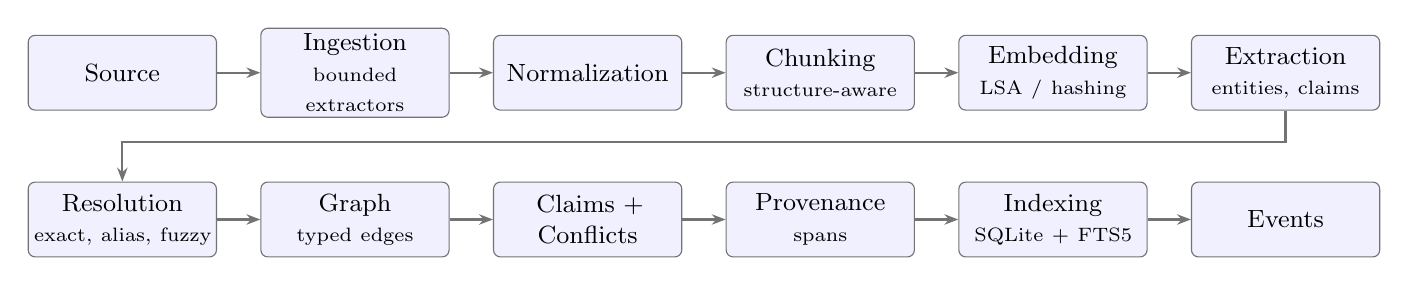
\begin{tikzpicture}[
  stage/.style={draw=black!55, rounded corners=2.5pt, text width=2.25cm,
                minimum height=0.95cm, align=center, font=\small,
                fill=blue!6, inner sep=2pt},
  arr/.style={-{Stealth[length=5pt]}, thick, black!55}
]
  % Row A: stages 1-6
  \node[stage] (n1) {Source};
  \node[stage, right=0.55cm of n1] (n2) {Ingestion\\{\scriptsize bounded extractors}};
  \node[stage, right=0.55cm of n2] (n3) {Normalization};
  \node[stage, right=0.55cm of n3] (n4) {Chunking\\{\scriptsize structure-aware}};
  \node[stage, right=0.55cm of n4] (n5) {Embedding\\{\scriptsize LSA / hashing}};
  \node[stage, right=0.55cm of n5] (n6) {Extraction\\{\scriptsize entities, claims}};
  % Row B: stages 7-12
  \node[stage, below=0.9cm of n1] (n7) {Resolution\\{\scriptsize exact, alias, fuzzy}};
  \node[stage, right=0.55cm of n7] (n8) {Graph\\{\scriptsize typed edges}};
  \node[stage, right=0.55cm of n8] (n9) {Claims + Conflicts};
  \node[stage, right=0.55cm of n9] (n10) {Provenance\\{\scriptsize spans}};
  \node[stage, right=0.55cm of n10] (n11) {Indexing\\{\scriptsize SQLite + FTS5}};
  \node[stage, right=0.55cm of n11] (n12) {Events};
  % Flow
  \draw[arr] (n1) -- (n2);
  \draw[arr] (n2) -- (n3);
  \draw[arr] (n3) -- (n4);
  \draw[arr] (n4) -- (n5);
  \draw[arr] (n5) -- (n6);
  \draw[arr] (n6.south) -- ++(0,-0.4) -| (n7.north);
  \draw[arr] (n7) -- (n8);
  \draw[arr] (n8) -- (n9);
  \draw[arr] (n9) -- (n10);
  \draw[arr] (n10) -- (n11);
  \draw[arr] (n11) -- (n12);
\end{tikzpicture}}
\caption{Ingestion pipeline. Detailed treatment per stage appears in
Sections \ref{sec:embeddings} through \ref{sec:jobs}.}\label{fig:ingestion}
\end{figure}

\begin{figure}[htbp]
\centering
\resizebox{0.92\columnwidth}{!}{%
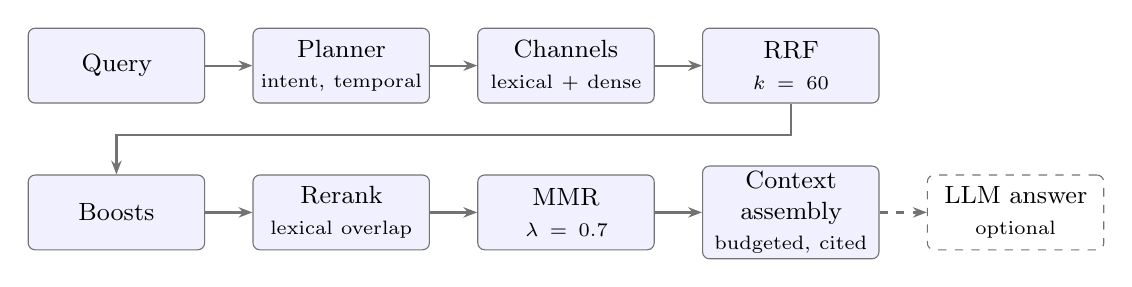
\begin{tikzpicture}[
  stage/.style={draw=black!55, rounded corners=2.5pt, text width=2.1cm,
                minimum height=0.95cm, align=center, font=\small,
                fill=blue!6, inner sep=2pt},
  opt/.style={stage, dashed, fill=none},
  arr/.style={-{Stealth[length=5pt]}, thick, black!55}
]
  % Row A
  \node[stage] (q1) {Query};
  \node[stage, right=0.6cm of q1] (q2) {Planner\\{\scriptsize intent, temporal}};
  \node[stage, right=0.6cm of q2] (q3) {Channels\\{\scriptsize lexical + dense}};
  \node[stage, right=0.6cm of q3] (q4) {RRF\\{\scriptsize $k=60$}};
  % Row B
  \node[stage, below=0.9cm of q1] (q5) {Boosts};
  \node[stage, right=0.6cm of q5] (q6) {Rerank\\{\scriptsize lexical overlap}};
  \node[stage, right=0.6cm of q6] (q7) {MMR\\{\scriptsize $\lambda=0.7$}};
  \node[stage, right=0.6cm of q7] (q8) {Context assembly\\{\scriptsize budgeted, cited}};
  \node[opt,   right=0.6cm of q8] (q9) {LLM answer\\{\scriptsize optional}};
  % Flow
  \draw[arr] (q1) -- (q2);
  \draw[arr] (q2) -- (q3);
  \draw[arr] (q3) -- (q4);
  \draw[arr] (q4.south) -- ++(0,-0.4) -| (q5.north);
  \draw[arr] (q5) -- (q6);
  \draw[arr] (q6) -- (q7);
  \draw[arr] (q7) -- (q8);
  \draw[arr, dashed] (q8) -- (q9);
\end{tikzpicture}}
\caption{Query pipeline. The dense channel is exact below the measured ANN
crossover and HNSW-served above it (Section~\ref{sec:ann}).}\label{fig:query}
\end{figure}

\subsection{Corpus-trained semantic embeddings}\label{sec:embeddings}

The provider interface is unchanged from v0.1 (\texttt{EmbeddingProvider});
v0.9 ships the real provider behind it:

\begin{enumerate}[itemsep=2pt]
\item \textbf{Vocabulary}: terms with document frequency $\geq$
\texttt{lsa\_min\_df}, capped at \texttt{lsa\_max\_vocab} by DF, totally
ordered (DF desc, then lexicographic) for determinism.
\item \textbf{Matrix}: per-chunk term counts weighted
$(1+\ln\mathrm{tf})\cdot\ln(1+N/\mathrm{df})$.
\item \textbf{Factorization}: randomized SVD with a fixed-seed Knuth LCG
sketch (Box--Muller Gaussians), 4 power iterations, modified Gram--Schmidt
orthonormalization, and a sign convention fixing each latent's largest
component positive.
\item \textbf{Encoding}: text $\rightarrow$ $\sum$ over in-vocabulary terms of
$(1+\ln\mathrm{tf})\cdot\mathit{term\_vector}$, L2-normalized; fully
out-of-vocabulary texts project to the zero vector (cosine 0 against
everything --- the lexical channel covers them; no fake similarity is
manufactured).
\item \textbf{Cold start}: below \texttt{semantic\_min\_chunks} the provider
\emph{is} the hashing embedder \cite{weinberger2009} and reports
\texttt{hashing-lex-v1} as its name. Above it, training is available via API
or job; the provider then reports \texttt{lsa-pmi-svd-v1}.
\end{enumerate}

Determinism is test-asserted: training twice on the same corpus yields
bit-identical vectors (\texttt{lsa\_training\_is\_deterministic}).

\subsection{Retrieval engine}\label{sec:retrieval}

Channels: BM25 (FTS5, prefix-AND sanitization), dense cosine (model-filtered,
single-pass), entity intersection (deterministic id-ordered). Fusion: RRF
$k=60$ with per-intent weights (Exact 0.25/0.75, Temporal 0.35/0.65, default
config 0.5/0.5). Boosts: positional authority (first chunks $1.2\times$, tail
$1.1\times$), exact phrase $+0.08$, known entity $+0.03$, section-title
overlap, freshness under \texttt{Latest} intent (re-rank, not filter ---
v0.1's hard filter could drop the newest evidence). Reranking: deterministic
lexical-overlap score (query-term coverage with length normalization) blended
50/50 with the fused score over the top-24 candidates --- the reranker can
only reorder channel-surfaced candidates, never inject unseen ones. Diversity:
MMR $\lambda=0.7$ with embeddings prefetched for the full candidate window
(cap 64). Every hit carries \texttt{matched\_by} evidence including its true
BM25 score.

\subsection{Claims and the conflict taxonomy}\label{sec:claims}

Three deterministic SVO families (numeric metrics, release/action verbs,
copula) produce claims with sentence offsets and temporal validity bounds
(since/from/as of/in $\rightarrow$ \texttt{valid\_from};
until/through/by $\rightarrow$ \texttt{valid\_until}). Negation is detected
and lowers confidence. Numeric objects are normalized through a magnitude
parser (\texttt{\$10 million} $\equiv$ \texttt{\$10M} $\equiv$ 10\,000\,000;
commas, \%, B/K handled; the parser scans left-to-right --- v0.1 kept only the
last token). Conflict detection compares against the most recent 40
same-metric claims (indexed lookup) and materializes at most 4 conflict rows
per claim --- disagreement \emph{existence} is the signal; full pair
enumeration is quadratic and uninformative (measured in
Section~\ref{sec:defects}). Each conflict carries a taxonomy kind and a
human-readable explanation with both validity periods.

\subsection{Entity resolution and the graph}\label{sec:entities}

Resolution stages: (1) canonical key (lowercase, legal-suffix stripped),
(2) alias table (includes user-supplied aliases via
\texttt{add\_entity\_alias}), (3) type-guarded Jaro--Winkler $\geq 0.93$ with
first-letter blocking, confidence-scaled. Merges are audited
(\texttt{entity\_merge\_log}) and recompute the affected subgraph. Graph
edges: \texttt{CO\_OCCURS\_WITH} (weight = co-mention chunks) and
predicate-typed \texttt{RELATES\_TO\_*} edges derived from claims. Deletion
correctness: removing a document recomputes all edges around its entities
from surviving mentions --- v0.1's stale-edge defect is closed and
test-asserted. Reads: one-hop neighborhoods, multi-hop BFS (depth $\leq 3$,
deduplicated), degree centrality.

\subsection{Incremental model migration}\label{sec:migration}

Each chunk records the embedding model that produced its vector
(\texttt{chunks.embedding\_model}, backfilled at migration). Training
installs a new model; \texttt{reembed\_stale\_chunks} migrates vectors in
batches of 256 with progress reporting and cooperative cancellation, at
22.9k chunks/s measured. Query-time dense search only compares vectors from
one model --- cross-model cosine is impossible by construction. Opening a
library whose recorded model identity cannot be restored (e.g., corrupted
\texttt{lsa\_terms}) fails with a typed \texttt{EmbeddingMismatch} error
rather than silently mixing spaces.

\subsection{Document intelligence}\label{sec:documents}

Bounded extractors: DOCX (OOXML \texttt{w:t} runs per paragraph), XLSX
(shared-strings + inline cells per row), PPTX (slide runs), EPUB (XHTML
spine), HTML/XML (script/style/head removal, block tags $\rightarrow$ line
breaks, named + numeric entity decoding), text/markdown/20+ code
languages/CSV/TSV/JSON. Guards: 64\,MiB raw cap, 256\,MiB decompressed cap
enforced with \texttt{take()} (not header trust), 4096-entry archive cap. PDF
is behind the \texttt{pdf} cargo feature (pure-Rust \texttt{pdf-extract}),
disabled by default to keep the dependency graph light; the error for a
disabled feature is explicit and actionable.

\subsection{Background engine}\label{sec:jobs}

Jobs are SQLite rows claimed atomically (immediate transaction + conditional
UPDATE --- v0.1's SELECT-then-UPDATE race is closed). Failures re-queue with
exponential backoff ($\mathit{base}\cdot 2^{\mathit{attempt}-1}$, capped,
release time \texttt{run\_at} --- hidden until due) and dead-letter after
\texttt{max\_attempts} with payload and error preserved. Cancellation is
cooperative (workers check between stages; pending jobs cancellable by id).
Progress is reported for long jobs (re-embed reports percentage).
\texttt{worker\_threads} is honored --- v0.1 recorded but ignored it.

\needspace{0.2\textheight}
\section{Evaluation Methodology}\label{sec:methodology}

\subsection{The failure of the v0.1 benchmark (self-criticism)}\label{sec:v1-failure}

v0.1's benchmark generated probe queries that echoed the generating
document's title tokens, then reported Recall@10 = 1.000. Because the probes
were lexically identical to the ground-truth document's most salient tokens,
the number carried no information about retrieval quality. Worse, the
synthetic corpus contained no sentences matching the claim extractor, so the
entire evidence layer produced zero artifacts (\texttt{claims 0,
conflicts 0}) and was never exercised end-to-end. We treat this as the
canonical example of circular evaluation and replaced it.

\subsection{Golden evaluation (graded qrels)}\label{sec:golden}

\texttt{tests/golden\_eval.rs} fixes a 16-document corpus (four topics
$\times$ four documents, two chunks each), 16 queries, and document-level
graded judgments (3 = directly answers, 2 = topical, 1 = marginal). Metrics:
Recall@5/10, MRR, nDCG@10 with graded gain $2^{g}-1$. The suite runs every
query in lexical-only, dense-only, and hybrid modes (ablation harness),
asserts honest floors: hybrid MRR no worse than 0.50, nDCG@10 no worse than
0.55, Recall@10 no worse than 0.85, and hybrid within 0.05 MRR of the best
single channel, and asserts rank reproducibility across independently
constructed engines.

\subsection{Adversarial suite}\label{sec:adversarial}

\texttt{tests/security\_hostile.rs} covers: oversize input at the cap,
invalid UTF-8, corrupt OOXML, decompression pressure, script/style leakage,
seven FTS-injection query shapes with post-attack index health checks,
Zalgo/emoji/control-character payloads, five-fold re-ingestion idempotency,
empty and 1\,MB queries, and graph correctness after deleting documents that
contributed the only evidence for specific edges.

\subsection{System benchmark}\label{sec:bench}

\texttt{lkos-bench} measures ingestion throughput, per-mode query latency
(p50\slash p95\slash p99), self-supervised retrieval sanity, and semantic
training and re-embedding throughput. It also measures the ANN dense-channel
crossover (brute vs HNSW build, latency, recall, and deletion across corpus
sizes) and library statistics.
Archived output: \texttt{benchmarks/results/v0.9.0-run1.txt},
\texttt{benchmarks/results/ann-crossover-v0.10.0.txt}.

\subsection{Test inventory}\label{sec:tests}

86 tests: 23 end-to-end engine invariants (incl.\ 2 migration-resilience
regressions), 19 unit-quality tests, 9 semantic-layer tests, 12 adversarial
tests, 2 golden-evaluation tests, 5 ANN integration tests (exactness,
invalidation, policy paths), 14 module unit tests (LSA\slash JW\slash temporal\slash HNSW),
2 doc tests. All pass in release mode on this machine; CI runs the same suite
on Linux\slash macOS\slash Windows.

% ─────────────────────────────────────────────────────────
% §5 Results (3 tables), §6 Defects
% ─────────────────────────────────────────────────────────

\needspace{0.2\textheight}
\section{Results}\label{sec:results}

\subsection{System benchmark (200 docs, 2,400 chunks, 1.07M chars)}\label{sec:sysbench}

\begin{table}[htbp]
\centering
\caption{System benchmark, v0.1 vs v0.9 (same corpus, same machine).}
\label{tab:sysbench}
\footnotesize
\begin{tabular*}{\columnwidth}{@{\extracolsep{\fill}} l l l}
\toprule
Metric & v0.1 (run1) & v0.9 (run1) \\
\midrule
Ingestion throughput & 8.0 docs/s & 6.3 docs/s\textsuperscript{*} \\
Lexical p50 / p99 & 2.49 / 3.1 ms & 3.47 / 4.94 ms \\
Dense p50 / p99 & 14.0 / -- ms (hashing, N+1) & 6.28 / 6.66 ms (LSA, single-pass) \\
Hybrid p50 / p99 & 14.8 / -- ms & 7.43 / 8.12 ms (RRF + rerank) \\
Claims extracted & 0 & 4,800 \\
Conflicts detected & 0 & 9,548 \\
Entities / mentions & 3,552 / 12,000 & 2,384 / 22,400 \\
LSA train / re-embed & -- & 0.06 s / 22.9k chunks/s \\
\bottomrule
\end{tabular*}

\vspace{0.35em}
\begin{minipage}{0.92\columnwidth}
\footnotesize\textsuperscript{*}\,v0.9 ingestion now extracts ${\sim}24$ claims per
document, runs indexed conflict detection, and builds 10.7k graph edges ---
strictly more work per document; the dense-channel speedup ($-55\%$ p50) comes
from replacing the N+1 blob fetch with one model-filtered scan.
\end{minipage}
\end{table}

\subsection{Golden evaluation (16 queries, graded judgments, hashing fallback active)}\label{sec:goldenresults}

\begin{table}[htbp]
\centering
\caption{Golden-set ablation across retrieval modes.}
\label{tab:golden}
\small
\begin{tabular*}{\columnwidth}{@{\extracolsep{\fill}} l c c c c}
\toprule
Mode & Recall@5 & Recall@10 & MRR & nDCG@10 \\
\midrule
Lexical only & 0.938 & 0.938 & 0.938 & 0.873 \\
Dense only & 1.000 & 1.000 & 1.000 & 0.966 \\
Hybrid (+rerank) & 1.000 & 1.000 & 1.000 & 0.966 \\
\bottomrule
\end{tabular*}
\end{table}

Interpretation, deliberately conservative: on a 16-document corpus with a
small vocabulary, feature hashing already produces usable topical geometry,
and fusion matches it while retaining lexical guarantees. The golden set's
purpose is regression protection and honest floor enforcement~--- \textbf{not}
claims of state-of-the-art retrieval. Its size is a documented limitation
(Section~\ref{sec:limitations}.5).

\subsection{What the tests prove}\label{sec:testsprove}

Beyond the evaluation numbers, 77 assertions encode behavioral contracts:
idempotent ingestion; changed-content versioning; deleted documents vanish
from documents, chunks, mentions, provenance \emph{and} the graph;
corrupted-model libraries refuse to open rather than mix embedding spaces;
\texttt{\$10 million} and \texttt{\$10M} do not conflict;
\texttt{\$10M}/2023 vs \texttt{\$25M}/2024 is classified cross-period while
same-period disagreement is classified as such; backed-off jobs are invisible
until release and dead-letter after exhaustion; cancelled jobs never claim;
five duplicate ingestions produce one document; the FTS index survives seven
injection shapes; the engine answers queries from four threads concurrently
with deterministic output.

\subsection{ANN crossover (v0.10)}\label{sec:ann}

Dense-channel comparison on a clustered 128-d corpus (40 topics, jitter 0.05;
queries jitter actual cluster centers --- the regime the dense channel
serves). $M=16$, efC$=200$; ground truth is the exact scan; all values
deterministic. Source: \texttt{benchmarks/results/ann-crossover-v0.10.0.txt}.

\begin{table}[htbp]
\centering
\caption{ANN crossover: brute force vs deterministic HNSW across corpus sizes.
Rebuild = delete-10\% rebuild (invalidation strategy: full rebuild, ADR-010).}
\label{tab:ann}
\small
\begin{tabular*}{\columnwidth}{@{\extracolsep{\fill}} l c cc cc c c}
\toprule
 & & \multicolumn{2}{c}{ANN ef=64} & \multicolumn{2}{c}{ANN ef=128} & & \\
\cmidrule(lr){3-4}\cmidrule(lr){5-6}
$N$ & Brute p50 & p50 & R@10 & p50 & R@10 & Build & Rebuild \\
\midrule
1,000 & 0.17 ms & 0.046 ms & 1.000 & 0.082 ms & 1.000 & 0.14 s & 0.12 s \\
5,000 & 0.99 ms & 0.051 ms & 1.000 & 0.079 ms & 1.000 & 0.80 s & 0.72 s \\
20,000 & 3.81 ms & 0.115 ms & 0.997 & 0.149 ms & 1.000 & 3.9 s & 3.4 s \\
50,000 & 10.01 ms & 0.197 ms & 0.960 & 0.294 ms & 0.993 & 15.0 s & 12.7 s \\
100,000 & 20.24 ms & 0.296 ms & 0.853 & 0.415 ms & 0.967 & 46.4 s & 40.4 s \\
\bottomrule
\end{tabular*}
\end{table}

Reading, deliberately conservative: the ANN path buys 34--87$\times$ dense p50
at this scale but is \emph{approximate} --- the default
\texttt{ann\_ef\_search}$=64$ holds recall@10 $\geq 0.95$ through ${\sim}50$k
chunks on this corpus, and ef$=128$ through ${\sim}50$k at $\geq 0.99$ with
0.967 at 100k. Break-even (build amortized against per-query savings) sits at
${\sim}1.1$k--2.3k dense queries, which is why \texttt{auto} keeps the exact
scan below \texttt{ann\_min\_chunks} $= 20{,}000$ and why the engine caches
the index across queries. Deletion is quantified as full-rebuild cost
($\approx 0.87\times$ one build) --- the fingerprint makes the rebuild
\emph{correct}; a serialized incremental graph is registered future work, not
claimed.

Two defects surfaced only because the harness measured recall against exact
ground truth; both are recorded in Section~\ref{sec:defects} (items 11--12)
with their fixes.

\needspace{0.2\textheight}
\section{Defects Found by the Audit (and Fixed)}\label{sec:defects}

The adversarial process found nine defects that v0.1's functional tests had
missed; a tenth surfaced afterwards through the repository's own Windows CI
gate:

\begin{enumerate}[itemsep=3pt]
\item \textbf{Entity-regex greediness} --- ``Omega Corp partnered with Tau
Corp'' extracted as a single organization. Fixed by truncation at the first
legal-suffix boundary; regression-tested.
\item \textbf{Regex alternation order} --- \texttt{[MBKm\%]} matched the
\texttt{m} of ``million'', so ``\$10 million'' parsed as 10, creating a false
100\% conflict with ``\$10M''. Fixed by ordering longer alternatives first.
\item \textbf{Quadratic conflict materialization} --- 2,400 numeric claims
$\rightarrow$ ${\sim}500$k pairwise conflict rows, stalling ingestion.
Bounded (40-comparison window, 4 rows/claim) with rationale documented.
\item \textbf{NULL-intolerant neighbor reads} --- rebuilt graph edges (no
\texttt{last\_document\_id}) were silently dropped by \texttt{filter\_map} on
a type error, making post-delete neighborhoods empty. Found by the
graph-correct-deletion test; fixed with \texttt{Option<i64>}.
\item \textbf{Stale-edge deletion} --- v0.1 never cleaned co-occurrence
edges; deleting a document left permanent phantom relations. Fixed via
subgraph recompute.
\item \textbf{\texttt{embedding\_dim} ignored} --- v0.1 recorded the
configured dimension while hardcoding 256, so a library could lie about its
own geometry. Fixed; mismatch is now a typed error.
\item \textbf{\texttt{worker\_threads} dead} --- recorded but never used. Now
honored.
\item \textbf{Backoff/cancellation absent} --- failed jobs requeued
immediately and could not be cancelled; deadline-free retry loops were
possible. Fixed with \texttt{run\_at} + dead-letter + cooperative
cancellation.
\item \textbf{FTS score discarded} --- every lexical hit reported
\texttt{bm25: 0.0}, making score-based explanation impossible. Fixed (score
preserved, higher-is-better normalized).
\item \textbf{Migration stamps were not crash-atomic} (found by the project's
own Windows CI runner, post-v0.9). \texttt{user\_version} was stamped once
after \emph{all} batches, and scratch databases were named by wall-clock
timestamp --- whose effective granularity on Windows let two parallel tests
open the same fresh scratch file and migrate it concurrently, failing with
\texttt{duplicate column name: knowledge\_json}. A crash between batches
could likewise leave a fully-migrated library with a stale stamp that could
never reopen. Fixed in three layers: per-batch version stamps;
signature-column self-healing (a batch whose signature column already exists
is skipped, recovering stale-stamped databases); and process-unique scratch
paths (pid + atomic counter). Regression-tested
(\texttt{migration\_self\_heals\_when\_version\_stamp\_lags},
\texttt{parallel\_in\_memory\_engines\_are\_isolated}).
\item \textbf{HNSW result-heap ordering was inverted} (found by the v0.10
crossover harness, pre-release). The kept-results heap used a reversed
\texttt{Ord}, so its overflow \texttt{pop()} evicted the \emph{best} candidate
and the stop/accept gates compared against the best instead of the worst ---
measured recall@10 collapsed to 0.54 on a 2,000-node clustered corpus. Fixed
by defining \texttt{Ord} forward on the kept-results entry (\texttt{peek()} =
worst kept, \texttt{pop()} = evict worst) and reversed on the frontier entry
(\texttt{pop()} = nearest); the heap contract is now documented on the types
and locked by the exactness test (ef $\geq N$ must reproduce the brute-force
ranking).
\item \textbf{Ascending-id insertion starved cross-cluster bridges} (found by
the same harness at scale). Inserting nodes in id order on a
cluster-sequential corpus built isolated per-cluster subgraphs; recall
\emph{saturated} independent of ef (0.937 at ef $\geq 256$ on a 100k probe) ---
the signature of unreachable nodes, not insufficient search width. Fixed with
a deterministic hash-order insertion shuffle (splitmix64 of the chunk id),
which interleaves clusters from the first inserts; recall now scales smoothly
with ef (0.987 @ ef=128, 1.000 @ ef=512 on the probe corpus).
\end{enumerate}

% ─────────────────────────────────────────────────────────
% §7 Limitations, §8 Research Frontier, §9 Conclusion, References
% ─────────────────────────────────────────────────────────

\needspace{0.2\textheight}
\section{Limitations (Precise)}\label{sec:limitations}

\begin{enumerate}[itemsep=3pt]
\item \textbf{Embedding semantics are corpus-relative.}
LSA captures the distributional structure of \emph{this} library. It will not
transfer external synonyms (``car'' $\leftrightarrow$ ``automobile'' converge
only if the corpus evidences it). Paraphrase transfer requires a pretrained
encoder (ONNX/fastembed slot, ADR-005) --- not implemented, not claimed.
\item \textbf{Entity/claim extraction is deterministic regexing.}
No NER, no coreference, no NLI. Precision is conservative by design
(type-guarded linking, threshold 0.93); recall is unmeasured against NER
baselines --- future work (Section~\ref{sec:frontier}).
\item \textbf{Dense search is approximate above the crossover.}
v0.10 replaces the v0.9 refuse-past-cap behaviour with a deterministic HNSW
path \cite{malkov2018} (ADR-010): exact scan below \texttt{ann\_min\_chunks}
(20k) and under filters; ANN above. Approximate results are bounded by
measurement (recall@10 $\geq 0.95$ at ef=64 on the crossover corpus up to 50k
chunks; see Section~\ref{sec:ann}), not by guarantee. \emph{Persisted} ANN
graphs (serializing the index beside SQLite) remain future work ---
rebuild-after-mutation is the amortized v0.10 strategy.
\item \textbf{\texttt{open\_in\_memory} is a scratch file}, not
\texttt{:memory:} --- cleaned on \texttt{close()}, but not memory-resident.
\item \textbf{Golden set is small.}
16 queries guard regressions; they do not establish ranking superiority over
any external baseline. BEIR-style evaluation is future work.
\item \textbf{HTML extraction is structural, not reader-mode.} Boilerplate
(nav, ads) is not classified; templates are preserved as text.
\item \textbf{No OCR.} Scanned PDFs error with an actionable message.
\item \textbf{Bitemporality is partial.} Claims carry validity intervals;
chunk-level event time vs ingestion time is not yet separated at query time.
\end{enumerate}

\needspace{0.2\textheight}
\section{Research Frontier (Ordered by Expected Value)}\label{sec:frontier}

\begin{enumerate}[itemsep=3pt]
\item \textbf{BEIR-style external evaluation} --- measure hybrid/rerank
ablations on a public retrieval benchmark (licensing permitting) to replace
small-corpus floors with population-grade numbers.
\item \textbf{HNSW/IVF ANN} with measured recall/latency/build/update
crossover against the brute-force path, including deletion behavior. ---
\textbf{Delivered in v0.10} for the in-process case (ADR-010 +
\texttt{benchmarks/results/ann-crossover-v0.10.0.txt}). Remaining:
persisted/serialized graphs, IVF comparison at extreme N, streaming insertion
between rebuilds.
\item \textbf{Pretrained local encoders} via the existing
\texttt{EmbeddingProvider} trait (ONNX Runtime, fastembed models), with the
same model-lineage migration machinery LSA already exercises.
\item \textbf{Cross-encoder reranking} behind the same evidence-gated
ablation harness (adopt only if the golden/BEIR deltas justify the latency).
\item \textbf{NER-grade extraction} (small local models) replacing regex
entity/claim extraction, evaluated on a labeled slice of the golden corpus.
\item \textbf{Bitemporal query semantics} over claim validity intervals
(``what was true in 2023?'' answered structurally).
\end{enumerate}

\needspace{0.2\textheight}
\section{Conclusion}\label{sec:conclusion}

LKOS v0.9 demonstrates that a local-first knowledge engine can have real
semantic retrieval, a typed evidence layer, and graph-correct incremental
maintenance without a network, a GPU, or a bundled model --- and that its
quality claims can be made falsifiable: every architectural statement in this
paper corresponds to either a passing test, an archived measurement, or an
explicitly labeled limitation. The repository's own history is the strongest
evidence of the method: the adversarial audit converted nine silent defects
into nine regression tests. The finish line remains unchanged --- LKOS must be
infrastructure that other software can embed, query, update, observe, and
build upon --- and v0.9 moves it from ``specification ahead of
implementation'' to ``implementation that documents itself against
measurement''.

\begin{thebibliography}{11}

\bibitem{deerwester1990}
S.~Deerwester, S.~Dumais, G.~Furnas, T.~Landauer, and R.~Harshman,
``Indexing by latent semantic analysis,'' \emph{Journal of the American
Society for Information Science}, vol.~41, no.~6, 1990.

\bibitem{halko2011}
N.~Halko, P.-G.~Martinsson, and J.~Tropp, ``Finding structure with
randomness: Probabilistic algorithms for constructing approximate matrix
decompositions,'' \emph{SIAM Review}, vol.~53, no.~2, 2011.

\bibitem{robertson2009}
S.~Robertson and H.~Zaragoza, ``The probabilistic relevance framework: BM25
and beyond,'' \emph{Foundations and Trends in Information Retrieval},
vol.~3, no.~4, 2009.

\bibitem{cormack2009}
G.~Cormack, C.~Clarke, and S.~Buettcher, ``Reciprocal rank fusion outperforms
Condorcet and individual rank learning methods,'' in \emph{Proc.\ SIGIR},
2009.

\bibitem{carbonell1998}
J.~Carbonell and J.~Goldstein, ``The use of MMR, diversity-based reranking
for reordering documents and producing summaries,'' in \emph{Proc.\ SIGIR},
1998.

\bibitem{weinberger2009}
K.~Weinberger et~al., ``Feature hashing for large scale multitask learning,''
in \emph{Proc.\ ICML}, 2009.

\bibitem{winkler1989}
W.~Winkler, ``String comparator metrics and enhanced decision rules in the
Fellegi--Sunter model of record linkage,'' in \emph{ASA Survey Research
Methods}, 1989.

\bibitem{kleppmann2017}
M.~Kleppmann, \emph{Designing Data-Intensive Applications}. O'Reilly, 2017.

\bibitem{lewis2020}
P.~Lewis et~al., ``Retrieval-augmented generation for knowledge-intensive NLP
tasks,'' in \emph{Proc.\ NeurIPS}, 2020.

\bibitem{karpukhin2020}
V.~Karpukhin et~al., ``Dense passage retrieval for open-domain question
answering,'' in \emph{Proc.\ EMNLP}, 2020.

\bibitem{malkov2018}
Y.~Malkov and D.~Yashunin, ``Efficient and robust approximate nearest
neighbor search using Hierarchical Navigable Small World graphs,''
\emph{IEEE Transactions on Pattern Analysis and Machine Intelligence},
vol.~42, no.~4, pp.~824--836, 2018.

\end{thebibliography}


\end{document}
